\section{Resultados}
\label{sec:resultados}

A Tabela~\ref{tab:resultados} apresenta as métricas da última época dos
quatro experimentos, após 10 épocas de treinamento. Os valores de
acurácia são apresentados em porcentagem.

\begin{table}[ht]
  \centering
  \caption{Resultados de teste após 10 épocas.}
  \label{tab:resultados}
  \begin{tabular}{lrrr}
    \hline
    Experimento & \shortstack{Teste\\Top-1 (\%)} & \shortstack{Teste\\Top-5 (\%)} &
      \shortstack{Perda\\de teste} \\
    \hline
    Modelo de referência & 72,78 & 92,35 & 0,9959 \\
    BN estatístico & 58,04 & 81,94 & 1,6488 \\
    BN treinável & 78,93 & 94,74 & 0,7567 \\
    BN treinável + SD & 79,43 & 94,86 & 0,7362 \\
    \hline
  \end{tabular}
\end{table}

O experimento BN treinável + SD apresentou as maiores acurácias
e a menor perda de teste. Sua acurácia top-1 superou a do
modelo de referência em 6,65 pontos percentuais e a de
BN treinável em 0,50 ponto percentual. Sem Stochastic
Depth, BN treinável obteve um ganho de 6,15 pontos
percentuais sobre o modelo de referência. A atualização apenas
das estatísticas do Batch Normalization, em BN estatístico, apresentou
uma redução de 14,73 pontos percentuais em relação ao modelo de referência.
A ordenação das configurações pela acurácia top-1 foi a mesma na validação
e no teste.

A Figura~\ref{fig:metricas-validacao} apresenta a evolução da perda e das
acurácias top-1 e top-5 de validação ao longo das 10 épocas para as quatro
configurações.

\begin{figure}[ht]
  \centering
  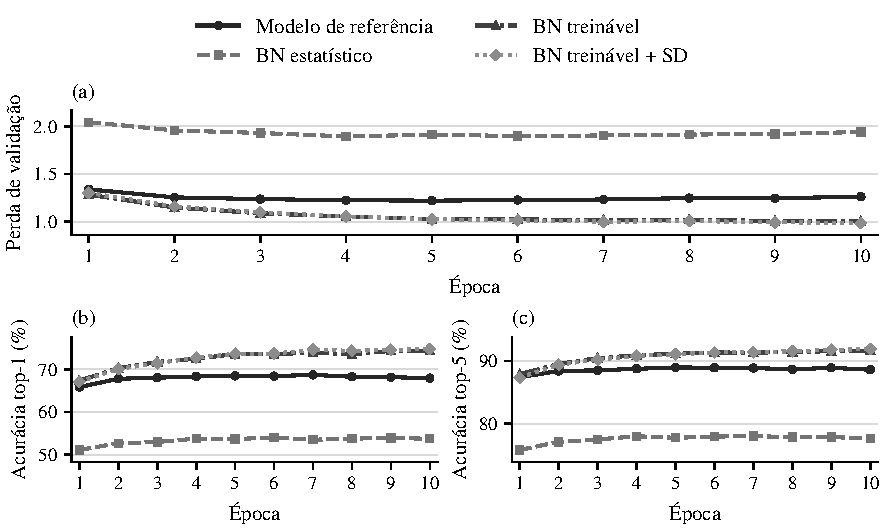
\includegraphics[width=\textwidth]{figures/metricas_validacao.pdf}
  \caption{Métricas de validação por época: (a) perda, (b) acurácia top-1 e
    (c) acurácia top-5. A legenda é compartilhada pelos três painéis.}
  \label{fig:metricas-validacao}
\end{figure}
